\documentclass[14pt,a4paper]{extarticle}
\usepackage{fontspec}
\IfFontExistsTF{Times New Roman}{\setmainfont{Times New Roman}}{\setmainfont{FreeSerif}}
\IfFontExistsTF{Consolas}{\setmonofont{Consolas}[Scale=0.85]}{\setmonofont{FreeMono}[Scale=0.85]}
\usepackage[russian]{babel}
\usepackage[left=30mm,right=15mm,top=20mm,bottom=20mm]{geometry}
\usepackage{amsmath,amssymb,graphicx,booktabs,array,longtable}
\usepackage{setspace,indentfirst,float,caption,listings,xcolor}
\usepackage[unicode,hidelinks]{hyperref}
\usepackage{titlesec}
\XeTeXgenerateactualtext=1
\setstretch{1.25}
\setlength{\parindent}{1.25cm}
\setlength{\emergencystretch}{2em}
\clubpenalty=10000
\widowpenalty=10000
\brokenpenalty=10000
\titleformat{\section}{\normalfont\large\bfseries}{\thesection}{0.7em}{}
\titleformat{\subsection}{\normalfont\normalsize\bfseries}{\thesubsection}{0.7em}{}
\captionsetup{font=small,labelsep=period}
\addto\captionsrussian{\renewcommand{\contentsname}{СОДЕРЖАНИЕ}}
\lstset{basicstyle=\ttfamily\footnotesize,breaklines=true,columns=fullflexible,
 keepspaces=true,showstringspaces=false,upquote=true,frame=none,aboveskip=0.6em,belowskip=0.6em}
\lstset{literate={-}{{\char45}}1}
\newcommand{\code}[1]{\texttt{\detokenize{#1}}}
\newcommand{\StudentName}{Антипенко С. В.}
\newcommand{\StudentGroup}{\underline{\hspace{2cm}}}
\newcommand{\TeacherName}{Лукашин А. А.}

\begin{document}
\begin{titlepage}
\begin{center}
\textbf{МИНИСТЕРСТВО НАУКИ И ВЫСШЕГО ОБРАЗОВАНИЯ РФ}

\vspace{0.4cm}
\textbf{Федеральное государственное автономное образовательное учреждение высшего образования}

\vspace{0.4cm}
\textbf{«Санкт-Петербургский политехнический университет Петра Великого»}

\vspace{0.6cm}
Высшая школа интеллектуальных систем и суперкомпьютерных технологий

\vfill
\textbf{ОТЧЁТ}

\vspace{0.3cm}
о выполнении практической работы

\vspace{0.5cm}
по дисциплине «Параллельное программирование на суперкомпьютерах»

\vspace{0.7cm}
\textbf{«Построение кубического сплайна»}

\vspace{0.3cm}
Вариант 24
\end{center}
\vspace{0.5cm}
\noindent\textbf{Выполнил:}\\[0.2cm]
студент группы \StudentGroup\hfill\StudentName
\begin{flushright}\small подпись\end{flushright}
\noindent\textbf{Проверил:}\\[0.2cm]
\TeacherName\hfill\underline{\hspace{3cm}}
\begin{flushright}\small подпись\end{flushright}
\vspace{0.3cm}
\begin{flushright}«\underline{\hspace{0.7cm}}» \underline{\hspace{3cm}} 2026 г.\end{flushright}
\vfill
\begin{center}Санкт-Петербург, 2026\end{center}
\end{titlepage}
\setcounter{page}{2}

\tableofcontents
\clearpage
\section{Введение}
Цель работы - реализовать построение кубического интерполяционного сплайна четырьмя способами и исследовать эффективность распараллеливания на суперкомпьютере. Для управления заданиями использован Slurm. Разработаны реализации C и Linux Pthreads, C и OpenMP, C и MPI, Python и MPI.

В отсутствие дополнительных требований к граничным условиям выбран натуральный кубический сплайн: его вторые производные на концах равны нулю. Корректность проверена относительно независимого эталона SciPy. Для потоковых версий число исполнителей изменялось от 1 до 48, для MPI - от 1 до 112. Эксперименты выполнены 11-12 ноября 2026 года под учётной записью \code{tm3u20}.

\section{Порядок выполнения работы}
\subsection{Подключение к кластеру}
Работа выполнена с использованием двух окон PowerShell. В первом окне установлено SSH-соединение с суперкомпьютером и выполнены серверные команды. Во втором окне выполнены локальные операции Windows и передача файлов. Ниже приведены использованные операции и соответствующие команды без символов приглашения оболочки.

\paragraph{1. Подключение к управляющему серверу.}
На персональном компьютере открыто первое окно PowerShell через Win+R и команду \code{powershell}. Подключение выполнено следующей командой:
\par\noindent\begin{minipage}{\linewidth}
\begin{lstlisting}
ssh -i "$env:USERPROFILE\.ssh\id_ed25519" tm3u20@login1.hpc.spbstu.ru
\end{lstlisting}
\end{minipage}\par
Для аутентификации использован SSH-ключ \code{id_ed25519}. После входа в терминале отобразилось приглашение \code{tm3u20@login1}. Ключ сервера был принят при первоначальном подключении.

\paragraph{2. Получение информации о сервере и очереди.}
После подключения в первом окне последовательно выполнены команды:
\par\noindent\begin{minipage}{\linewidth}
\begin{lstlisting}
hostname
whoami
sinfo
squeue -u "$USER"
\end{lstlisting}
\end{minipage}\par
Получены имя сервера \code{login1.cluster}, имя пользователя \code{tm3u20} и список разделов кластера. Первоначальный вывод \code{squeue} содержал только заголовок таблицы, то есть активных заданий не было. Состояние \code{idle} в выводе \code{sinfo} обозначало свободные узлы.

\subsection{Вводная лабораторная: узел, JSON и Python}
\paragraph{3. Интерактивное выделение вычислительного узла.}
В первом окне на управляющем сервере выделение ресурсов выполнено с помощью \code{salloc}. Команда имеет следующий вид:
\par\noindent\begin{minipage}{\linewidth}
\begin{lstlisting}
salloc -N1 -p cascade --ntasks=1 --cpus-per-task=4 --time=00:20:00
\end{lstlisting}
\end{minipage}\par
После ожидания ресурсов получено подтверждение выделения. Параметры приведённой команды задают один узел раздела \code{cascade}, четыре CPU и ограничение времени 20 минут. Номер задания и имя выделенного узла определены командами:
\par\noindent\begin{minipage}{\linewidth}
\begin{lstlisting}
echo "$SLURM_JOB_ID"
scontrol show hostnames "$SLURM_JOB_NODELIST"
\end{lstlisting}
\end{minipage}\par
Первая команда вывела номер текущего задания, вторая - имя выделенного узла. Значения этих параметров назначаются планировщиком при каждом выделении ресурсов.

\paragraph{4. Переход на вычислительный узел.}
Переход на выделенный узел выполнен по SSH. В следующем варианте команды имя узла автоматически определяется из текущего выделения Slurm:
\par\noindent\begin{minipage}{\linewidth}
\begin{lstlisting}
ssh "$(scontrol show hostnames "$SLURM_JOB_NODELIST" | head -n 1)"
\end{lstlisting}
\end{minipage}\par
После перехода имя узла и учётная запись проверены командами:
\par\noindent\begin{minipage}{\linewidth}
\begin{lstlisting}
hostname
whoami
\end{lstlisting}
\end{minipage}\par
При первоначальном выполнении вводной части команда \code{hostname} вывела \code{n06p049}. Таким образом подтверждён переход с управляющего сервера на вычислительный узел. Первое окно использовалось далее для работы на этом узле.

\paragraph{5. Создание локального JSON-файла.}
На персональном компьютере открыто второе окно PowerShell. Локальные команды выполнены вне SSH-сеанса, при приглашении вида \code{PS C:\Users\Admin>}. Создание каталога и входного файла задаётся следующим блоком:
\par\noindent\begin{minipage}{\linewidth}
\begin{lstlisting}
$introDir = Join-Path $env:USERPROFILE "Documents\spline-intro"
New-Item -ItemType Directory -Force -Path $introDir | Out-Null
Set-Location $introDir
'{"matrix": [[1, 2, 3], [4, 5, 6]]}' | Set-Content -Encoding ascii input.json
Get-Content .\input.json
\end{lstlisting}
\end{minipage}\par
Блок создаёт рабочий каталог \code{Documents\spline-intro}, записывает матрицу в \code{input.json} и выводит содержимое файла. Исходный JSON сформирован на персональном компьютере.

\paragraph{6. Передача входного файла через SCP.}
Передача файла выполнена во втором, локальном окне из каталога с \code{input.json}:
\par\noindent\begin{minipage}{\linewidth}
\begin{lstlisting}
scp -i "$env:USERPROFILE\.ssh\id_ed25519" .\input.json tm3u20@login1.hpc.spbstu.ru:~/input.json
\end{lstlisting}
\end{minipage}\par
После завершения передачи содержимое файла проверено в первом окне на вычислительном узле:
\par\noindent\begin{minipage}{\linewidth}
\begin{lstlisting}
cat ~/input.json
\end{lstlisting}
\end{minipage}\par
Домашний каталог доступен с управляющего и вычислительного узлов. На вычислительном узле прочитана переданная матрица \code{[[1, 2, 3], [4, 5, 6]]}.

\paragraph{7. Создание Python-скрипта.}
В первом окне на вычислительном узле подключён модуль Python:
\par\noindent\begin{minipage}{\linewidth}
\begin{lstlisting}
module load python/3.10
\end{lstlisting}
\end{minipage}\par
Создан скрипт \code{transpose.py}. Полный блок создания файла приведён ниже; строка \code{PY} завершает многострочный ввод:
\par\noindent\begin{minipage}{\linewidth}
\begin{lstlisting}
cat > ~/transpose.py <<'PY'
import json
from pathlib import Path

source = Path.home() / "input.json"
target = Path.home() / "output.json"
data = json.loads(source.read_text(encoding="utf-8"))
matrix = data["matrix"]
assert matrix and matrix[0], "Empty matrix"
assert all(len(row) == len(matrix[0]) for row in matrix), "Ragged matrix"
result = {"matrix": [list(row) for row in zip(*matrix)]}
target.write_text(json.dumps(result, indent=2), encoding="utf-8")
print("Saved:", target)
PY
\end{lstlisting}
\end{minipage}\par
Скрипт читает JSON, проверяет непустоту и прямоугольность матрицы, транспонирует её и записывает результат. Использованы стандартные библиотеки Python \code{json} и \code{pathlib}; внешние зависимости для вводной части не потребовались.

\paragraph{8. Преобразование матрицы и запись результата.}
В первом окне на вычислительном узле выполнены запуск скрипта и просмотр выходного файла:
\par\noindent\begin{minipage}{\linewidth}
\begin{lstlisting}
python3 ~/transpose.py
cat ~/output.json
\end{lstlisting}
\end{minipage}\par
Скрипт вывел путь к сохранённому файлу. Команда \code{cat} показала JSON с транспонированной матрицей:
\begin{equation}
A=\begin{pmatrix}1&2&3\\4&5&6\end{pmatrix},\qquad
A^{\mathsf T}=\begin{pmatrix}1&4\\2&5\\3&6\end{pmatrix}.
\end{equation}

\paragraph{9. Передача результата на персональный компьютер.}
В локальном окне PowerShell из каталога \code{Documents\spline-intro} выполнены скачивание и просмотр результата:
\par\noindent\begin{minipage}{\linewidth}
\begin{lstlisting}
scp -i "$env:USERPROFILE\.ssh\id_ed25519" tm3u20@login1.hpc.spbstu.ru:~/output.json .\output.json
Get-Content .\output.json
\end{lstlisting}
\end{minipage}\par
Результат получен на персональном компьютере. В выходном файле сохранены строки матрицы \code{[1, 4]}, \code{[2, 5]}, \code{[3, 6]}.

\paragraph{10. Завершение работы и освобождение ресурсов.}
SSH-сеанс вычислительного узла завершён в первом окне командой:
\par\noindent\begin{minipage}{\linewidth}
\begin{lstlisting}
exit
\end{lstlisting}
\end{minipage}\par
После возвращения на \code{login1} выделение освобождено и выполнена проверка очереди. Для текущего задания используются команды:
\par\noindent\begin{minipage}{\linewidth}
\begin{lstlisting}
scancel "$SLURM_JOB_ID"
squeue -u "$USER"
\end{lstlisting}
\end{minipage}\par
Переменная \code{SLURM_JOB_ID} содержит номер задания в оболочке \code{salloc}. После освобождения ресурсов соответствующее задание исчезло из активной очереди. При истечении лимита времени ресурсы освобождаются планировщиком автоматически.

В результате выполнены подключение по SSH, получение информации о кластере и очереди, выделение узла, передача входного JSON, обработка матрицы Python-скриптом, получение \code{output.json} на персональном компьютере и освобождение ресурсов.

Первоначально вводная часть выполнена в задании 9261607 на \code{n06p049}. В приведённых командах используются параметры текущего выделения Slurm, поэтому имя вычислительного узла не зафиксировано в командах подключения.

\subsection{Подготовка проекта и сборка}
Каталог \code{spline-lab} передан на сервер командой \code{scp -r}. На управляющем сервере загружены доступные модули:
\begin{samepage}
\par\noindent\begin{minipage}{\linewidth}
\begin{lstlisting}
module load compiler/gcc/11 mpi/openmpi/4.1.6/gcc/11 python/3.10
python3 -m venv ~/spline-lab/.venv
source ~/spline-lab/.venv/bin/activate
python3 -m pip install -r ~/spline-lab/requirements.txt
cd ~/spline-lab
make -j3
\end{lstlisting}
\end{minipage}\par
\end{samepage}
Установлены NumPy, SciPy, mpi4py и Matplotlib. Три C-программы собраны из общего исходного файла с разными флагами:
\begin{samepage}
\par\noindent\begin{minipage}{\linewidth}
\begin{lstlisting}
gcc -O3 -std=c11 src/spline.c -pthread -lm -o bin/spline_pthreads
gcc -O3 -std=c11 -DUSE_OMP src/spline.c -fopenmp -pthread -lm -o bin/spline_openmp
mpicc -O3 -std=c11 -DUSE_MPI src/spline.c -pthread -lm -o bin/spline_mpi
\end{lstlisting}
\end{minipage}\par
\end{samepage}
Флаг \code{-O3} включает оптимизацию, \code{-pthread} подключает POSIX Threads, \code{-fopenmp} - поддержку OpenMP. Обёртка \code{mpicc} подключает MPI.

\subsection{Проверка и пакетные запуски}
В интерактивном задании 9261675 на узле \code{n06p049} выполнен \code{bash tests/correctness.sh}. Все четыре реализации прошли тестирование. Затем подготовлены пакетные сценарии:
\begin{samepage}
\par\noindent\begin{minipage}{\linewidth}
\begin{lstlisting}
mkdir -p logs results work
sbatch slurm/threads.sbatch
sbatch slurm/mpi.sbatch
\end{lstlisting}
\end{minipage}\par
\end{samepage}
Потоковому заданию 9261711 запрошен один узел \code{cascade}, одна задача и 48 CPU. MPI-заданию 9261714 запрошены четыре узла \code{tornado}, 112 задач, по 28 задач на узел. В сценариях загружаются те же модули и активируется виртуальное окружение Python.

Перед MPI-серией проверен обмен \code{allreduce} между двумя узлами. Из-за предупреждения инициализации OpenFabrics для воспроизводимости явно выбран транспорт:
\begin{samepage}
\par\noindent\begin{minipage}{\linewidth}
\begin{lstlisting}
export OMPI_MCA_pml=ob1
export OMPI_MCA_btl=self,vader,tcp
\end{lstlisting}
\end{minipage}\par
\end{samepage}
Внутри узла используются компоненты \code{self/vader}, между узлами - TCP. Конкретный физический интерфейс TCP не фиксировался; результаты не характеризуют нативный InfiniBand-транспорт.

\subsection{Контроль выполнения и обработка результатов}
После завершения проверены состояния заданий и созданы графики:
\begin{samepage}
\par\noindent\begin{minipage}{\linewidth}
\begin{lstlisting}
sacct -j 9261711,9261714 --format=JobID,State,Elapsed,AllocCPUS,NodeList%40,ExitCode -X
python3 scripts/plot.py
\end{lstlisting}
\end{minipage}\par
\end{samepage}
Оба задания имеют состояние \code{COMPLETED} и код выхода \code{0:0}. Продолжительность потокового задания - 1 мин 56 с, MPI - 5 мин 28 с. Скачанные файлы ошибок пусты. Результаты объединены в \code{results/benchmark.csv}, исходные журналы сохранены в каталоге \code{logs}.
\begin{figure}[H]
\centering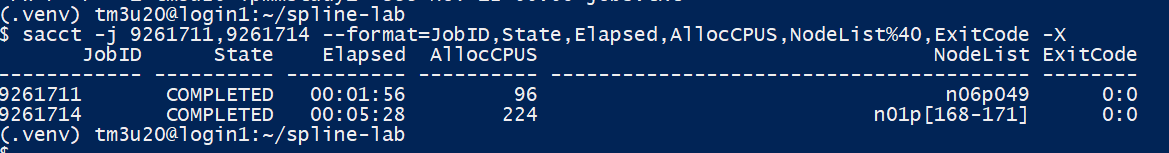
\includegraphics[width=\linewidth]{figures/jobs-completed.png}
\caption{Подтверждение завершения двух серий заданий Slurm}
\label{fig:jobs}
\end{figure}
Снимок \code{results/jobs.txt} был записан во время работы MPI и содержит промежуточное состояние. Окончательные состояния подтверждает рисунок~\ref{fig:jobs}.

\section{Постановка задачи}
Заданы конечные значения $y_i$ в строго возрастающих узлах $x_0<x_1<\dots<x_{n-1}$, $n\geq2$. На интервале $[x_i,x_{i+1}]$ требуется определить полином
\begin{equation}
S_i(x)=a_i+b_it+c_it^2+d_it^3,\qquad t=x-x_i.
\end{equation}
Условия интерполяции и гладкости:
\begin{align}
S_i(x_i)&=y_i,&S_i(x_{i+1})&=y_{i+1},\\
S'_{i-1}(x_i)&=S'_i(x_i),&S''_{i-1}(x_i)&=S''_i(x_i).
\end{align}
Для натурального сплайна дополнительно заданы
\begin{equation}
S''(x_0)=S''(x_{n-1})=0.
\end{equation}
Выход программы - четыре коэффициента для каждого из $n-1$ интервалов. Входной текстовый файл содержит количество узлов, затем пары $x_i,y_i$.

\section{Последовательный алгоритм и PCR}
Обозначим $h_i=x_{i+1}-x_i$, $M_i=S''(x_i)$. Для внутренних узлов выполняется трёхдиагональная система
\begin{equation}\label{eq:system}
\begin{split}
h_{i-1}M_{i-1}+2(h_{i-1}+h_i)M_i+h_iM_{i+1}\\
=6\left(\frac{y_{i+1}-y_i}{h_i}-\frac{y_i-y_{i-1}}{h_{i-1}}\right),
\end{split}
\end{equation}
где $1\leq i\leq n-2$, $M_0=M_{n-1}=0$. После решения системы коэффициенты вычисляются независимо:
\begin{align}
a_i&=y_i,\\
b_i&=\frac{y_{i+1}-y_i}{h_i}-\frac{h_i}{6}(2M_i+M_{i+1}),\\
c_i&=\frac{M_i}{2},\qquad
d_i=\frac{M_{i+1}-M_i}{6h_i}.
\end{align}

Последовательная прогонка решает систему за $O(n)$ операций при $O(n)$ памяти, но прямой и обратный ход содержат зависимости между соседними шагами. Возможные подходы к распараллеливанию - циклическая редукция, параллельная циклическая редукция (PCR), блочное исключение с отдельным решением системы на границах блоков.

В работе выбран PCR. На стадии с расстоянием $s=1,2,4,\dots$ из каждой строки исключаются неизвестные $M_{i-s}$ и $M_{i+s}$. Пусть текущая строка имеет коэффициенты $(A_i,B_i,C_i,D_i)$. Для существующих соседей вводятся
\begin{equation}
\alpha_i=-\frac{A_i}{B_{i-s}},\qquad
\beta_i=-\frac{C_i}{B_{i+s}}.
\end{equation}
Новая строка вычисляется по формулам
\begin{align}
A'_i&=\alpha_i A_{i-s},\\
B'_i&=B_i+\alpha_i C_{i-s}+\beta_i A_{i+s},\\
C'_i&=\beta_i C_{i+s},\\
D'_i&=D_i+\alpha_i D_{i-s}+\beta_i D_{i+s}.
\end{align}
Вклады отсутствующих соседей равны нулю. Строки одной стадии независимы и вычисляются из старого буфера в новый. Между стадиями выполняется синхронизация. После $\lceil\log_2n\rceil$ стадий $M_i=D_i/B_i$.

Суммарная работа PCR составляет $O(n\log n)$, число стадий - $O(\log n)$, память - $O(n)$. PCR выполняет больше арифметики, чем прогонка. Поэтому ускорение относительно однопоточного PCR не означает преимущество над оптимальной последовательной прогонкой; отдельное сравнение с ней в эксперименте не проводилось.

\section{Параллельные реализации}
\subsection{C и Linux Pthreads}
На один вызов решения создаётся пул из $p$ потоков. Строки распределяются циклически: поток с номером $r$ обрабатывает $r,r+p,r+2p,\dots$. Барьер разделяет соседние стадии PCR; ещё один барьер отделяет вычисление вторых производных от коэффициентов сплайна. Создание и завершение пула входят в измеряемое время.

Циклическое распределение соседних строк может приводить к совместному использованию строк кэша. Влияние этого эффекта отдельно не измерялось.

\subsection{C и OpenMP}
Единая параллельная область охватывает решение системы и построение коэффициентов. Используется \code{omp for schedule(static)}. Неявные барьеры и конструкция \code{single} обеспечивают готовность данных перед сменой буферов. Число потоков передаётся аргументом программы. В сценарии заданы \code{OMP_PROC_BIND=true} и \code{OMP_PLACES=cores}.

\subsection{C и MPI}
Строки распределяются непрерывными блоками. После вычисления локальных строк каждой стадии выполняется \code{MPI_Allgatherv}. Все процессы хранят полные массивы; после вычисления $M_i$ и коэффициентов также производится сбор данных.

Память на процесс равна $O(n)$. Репликация упрощает проверку, однако обмен полными массивами на каждой стадии ограничивает масштабирование. Более сложная распределённая редукция или блочный метод могут уменьшить объём обменов.

\subsection{Python и MPI}
Схема распределения и коллективных обменов совпадает с C/MPI. Межпроцессное взаимодействие реализовано через mpi4py, локальные арифметические операции - векторизованными средствами NumPy. Создание масок и временных массивов входит во время решения. Многопоточность BLAS в MPI-сценарии отключена.

Три C-программы собираются из \code{src/spline.c} с разными флагами препроцессора. Python-реализация находится в \code{src/spline_mpi.py}, общие численные функции - в \code{src/spline_math.py}.

\section{Тестирование корректности}
Независимым эталоном служит \code{scipy.interpolate.CubicSpline} с параметром \code{bc_type='natural'}~\cite{scipy}. Набор тестов приведён в таблице~\ref{tab:tests}. Каждая реализация проверена с 1, 2 и 4 исполнителями: всего 60 запусков.
\begin{table}[H]\centering
\caption{Набор тестов корректности}\label{tab:tests}
\small
\begin{tabular}{lrp{6.3cm}}\toprule
Тест & $n$ & Проверяемый случай\\\midrule
Две точки & 2 & Минимальный размер, $p>n$\\
Константа & 17 & Постоянная функция\\
Прямая & 33 & Линейная функция\\
Синус & 128 & Равномерная сетка\\
Неравномерная сетка & 129 & Различные расстояния между узлами\\\bottomrule
\end{tabular}
\end{table}
Проверяются коэффициенты относительно эталона, значения внутри интервалов, прохождение через исходные узлы, непрерывность первой и второй производных и нулевые вторые производные на концах. Критерий сравнения имеет вид
\begin{equation}
|v-v_{\mathrm{ref}}|\leq\varepsilon_{\mathrm{abs}}+
\varepsilon_{\mathrm{rel}}|v_{\mathrm{ref}}|.
\end{equation}
Для значений и производных $\varepsilon_{\mathrm{abs}}=\varepsilon_{\mathrm{rel}}=10^{-9}$, для коэффициентов - $10^{-7}$.

Полный сценарий завершился сообщением \code{ALL FOUR IMPLEMENTATIONS PASSED}. В последнем показанном тесте $n=129$, $p=4$ ошибка значения составила $6{,}2727600891321345\cdot10^{-15}$. Это ошибка конкретного теста, а не максимум по всему набору. Полный журнал исходного тестирования отдельно не сохранялся; результат зафиксирован в терминальном выводе.

Дополнительно выполнены проверочные запуски всех четырёх реализаций на узле \code{n06p048}: $n=129$, неравномерная сетка, четыре исполнителя. Результаты показаны на рисунках~\ref{fig:threads} и~\ref{fig:mpi}. Их времена не включены в основную серию измерений.
\begin{figure}[H]\centering
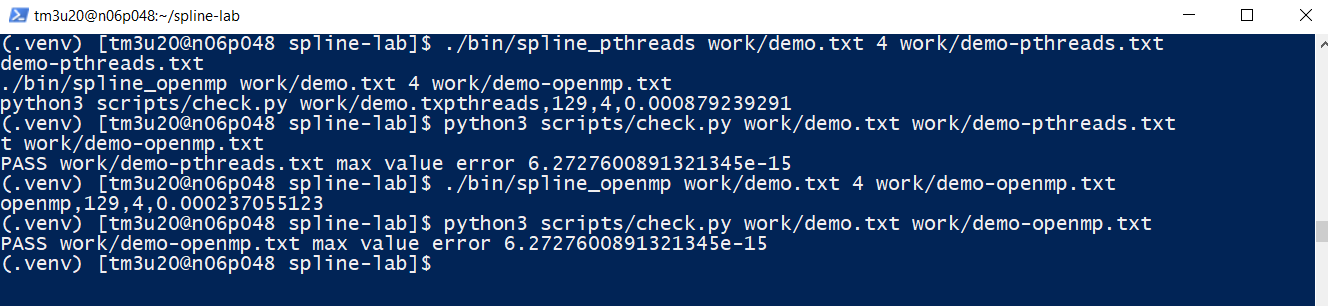
\includegraphics[width=\linewidth]{figures/demo-threads.png}
\caption{Проверка C/Pthreads и C/OpenMP: обе реализации получили PASS}
\label{fig:threads}
\end{figure}
\begin{figure}[H]\centering
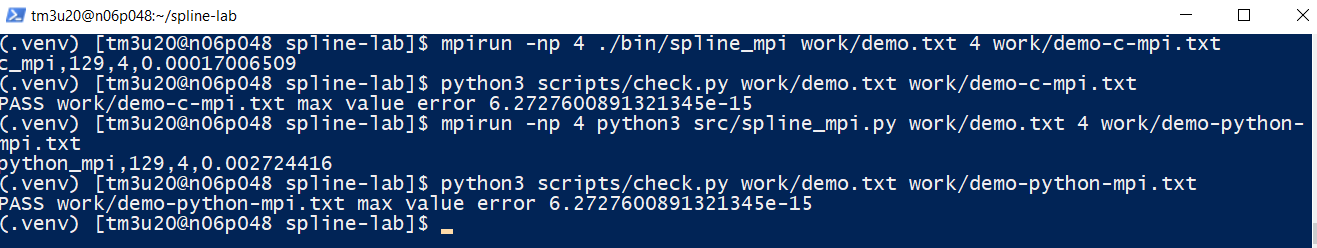
\includegraphics[width=\linewidth]{figures/demo-mpi.png}
\caption{Проверка C/MPI и Python/MPI: обе реализации получили PASS}
\label{fig:mpi}
\end{figure}
На локальном компьютере дополнительно проверены 96 случаев численных Python-функций относительно SciPy. Они дополняют, но не заменяют кластерные MPI-проверки. Скринкаст не записывался; в отчёте представлены скриншоты запусков.

\section{Методика вычислительного эксперимента}
\subsection{Оборудование и окружение}
Потоковые версии запускались в разделе \code{cascade} на \code{n06p049}: два Intel Xeon Gold 6248R, по 24 физических ядра на сокет, два аппаратных потока на ядро. Всего 48 физических ядер и 96 аппаратных потоков.

MPI-версии запускались на четырёх узлах \code{n01p168--171} раздела \code{tornado}, по 28 задач на узел. В проверенной выборке \code{sinfo} для этого раздела указаны 28 физических ядер и 56 аппаратных потоков на узел; модель CPU именно выделенных узлов отдельно не записана. При запуске использован \code{--bind-to core}. Подробная карта размещения рангов не сохранялась.

Для потокового задания Slurm показывает \code{AllocCPUS=96}, для MPI - \code{AllocCPUS=224}. Эти значения отражают выделение ресурсов с учётом SMT; фактическое число программных исполнителей задаётся аргументами программы и \code{mpirun -np}.

Применены модули GCC 11, Open MPI 4.1.6 и Python 3.10. Межузловые MPI-обмены выполнены через TCP; настройки транспорта одинаковы для всех MPI-конфигураций.

\subsection{Параметры и границы замера}
Исследованы три размера $n\in\{10\,000,100\,000,1\,000\,000\}$. Для каждого размера заданы равномерные узлы на $[0,20]$ и значения $y_i=\sin x_i$.

Для Pthreads и OpenMP использованы
\begin{equation}
p\in\{1,2,4,8,12,16,24,32,48\},
\end{equation}
для двух MPI-реализаций -
\begin{equation}
p\in\{1,2,4,8,16,28,56,84,112\}.
\end{equation}
Всего исследованы 108 конфигураций. Для каждой выполнены пять повторов в одном запуске; сохранялся минимум времени. Отдельные времена повторов в файлы не выводились, поэтому статистический разброс по сохранённым данным оценить нельзя.

Таймер исключает чтение и запись файлов, генерацию данных и формирование исходной системы. Включены PCR, вычисление коэффициентов и необходимые обмены; для Pthreads - создание и завершение пула, для MPI - служебные массивы распределения. В MPI для каждого повтора берётся максимум времени по процессам. Измеряется вычислительное ядро с указанными служебными расходами, а не полная длительность задания Slurm.

Ускорение и эффективность определяются как
\begin{equation}
S_p=\frac{T_1}{T_p},\qquad E_p=\frac{S_p}{p}.
\end{equation}
Время $T_1$ выбирается отдельно для каждой реализации и каждого размера задачи. Сравнение абсолютных времён между потоковыми и MPI-версиями ограничено различием оборудования.

\section{Результаты эксперимента}
Исходные журналы содержат по 54 строки для потоковой и MPI-серии. Все 108 конфигураций присутствуют; времена в CSV совпадают с журналами, ускорения и эффективность проверены повторным вычислением. Лучшие результаты среди проверенных $p$, включая $p=1$, приведены в таблицах~\ref{tab:best10000}-\ref{tab:best1000000}.

\begin{table}[H]\centering\small
\caption{Лучшие результаты при $n=10000$}\label{tab:best10000}
\begin{tabular}{lrrrrr}\toprule
Реализация & $T_1$, с & Лучшее $p$ & $T_p$, с & $S_p$ & $E_p$, \%\\\midrule
C + Pthreads & 0,000694 & 2 & 0,000674 & 1,030 & 51,49\\
C + OpenMP & 0,000609 & 24 & 0,000111 & 5,494 & 22,89\\
C + MPI & 0,001161 & 2 & 0,001047 & 1,109 & 55,44\\
Python + MPI & 0,018681 & 28 & 0,004711 & 3,965 & 14,16\\
\bottomrule\end{tabular}
\end{table}

\begin{table}[H]\centering\small
\caption{Лучшие результаты при $n=100000$}\label{tab:best100000}
\begin{tabular}{lrrrrr}\toprule
Реализация & $T_1$, с & Лучшее $p$ & $T_p$, с & $S_p$ & $E_p$, \%\\\midrule
C + Pthreads & 0,008892 & 32 & 0,004584 & 1,940 & 6,06\\
C + OpenMP & 0,008338 & 48 & 0,000528 & 15,785 & 32,89\\
C + MPI & 0,013330 & 2 & 0,011154 & 1,195 & 59,75\\
Python + MPI & 0,215794 & 16 & 0,053368 & 4,044 & 25,27\\
\bottomrule\end{tabular}
\end{table}

\begin{table}[H]\centering\small
\caption{Лучшие результаты при $n=1000000$}\label{tab:best1000000}
\begin{tabular}{lrrrrr}\toprule
Реализация & $T_1$, с & Лучшее $p$ & $T_p$, с & $S_p$ & $E_p$, \%\\\midrule
C + Pthreads & 0,140590 & 48 & 0,049335 & 2,850 & 5,94\\
C + OpenMP & 0,140010 & 48 & 0,010260 & 13,646 & 28,43\\
C + MPI & 0,199836 & 1 & 0,199836 & 1,000 & 100,00\\
Python + MPI & 3,595586 & 8 & 0,760502 & 4,728 & 59,10\\
\bottomrule\end{tabular}
\end{table}

При $n=1\,000\,000$ OpenMP достиг времени $0{,}0102605$~с на 48 потоках: $S_{48}=13{,}646$, $E_{48}=28{,}43\%$. Pthreads достиг $0{,}0493346$~с и ускорения $2{,}850$ на 48 потоках. Разница согласуется с отличиями распределения строк и расходами создания потоков; без профилирования влияние отдельных причин количественно не разделяется.

Python/MPI на миллионе точек показал лучший результат на восьми процессах: $0{,}760502$~с, ускорение $4{,}728$. C/MPI на этом размере не ускорился: минимум $0{,}199836$~с получен при одном процессе. На 112 процессах времена составили $1{,}45503$~с для C/MPI и $1{,}50294$~с для Python/MPI.

Для меньших размеров C/MPI дал небольшой выигрыш на двух процессах. Python/MPI достиг лучшего результата на 28 процессах при $n=10\,000$ и на 16 при $n=100\,000$. На 56 и более процессах время заметно увеличивается. Обмен полными массивами через Allgatherv и межузловой TCP ограничивают масштабирование. Точная связь с размещением процессов требует отдельного профилирования и карты рангов.

На малом размере Pthreads почти не масштабируется: лучший результат на двух потоках лишь на 3\% быстрее одного, а 48 потоков работают медленнее. Для OpenMP оптимум среди проверенных конфигураций при $n=10\,000$ равен 24 потокам, на больших размерах - 48.

\clearpage
\begin{figure}[p]\centering
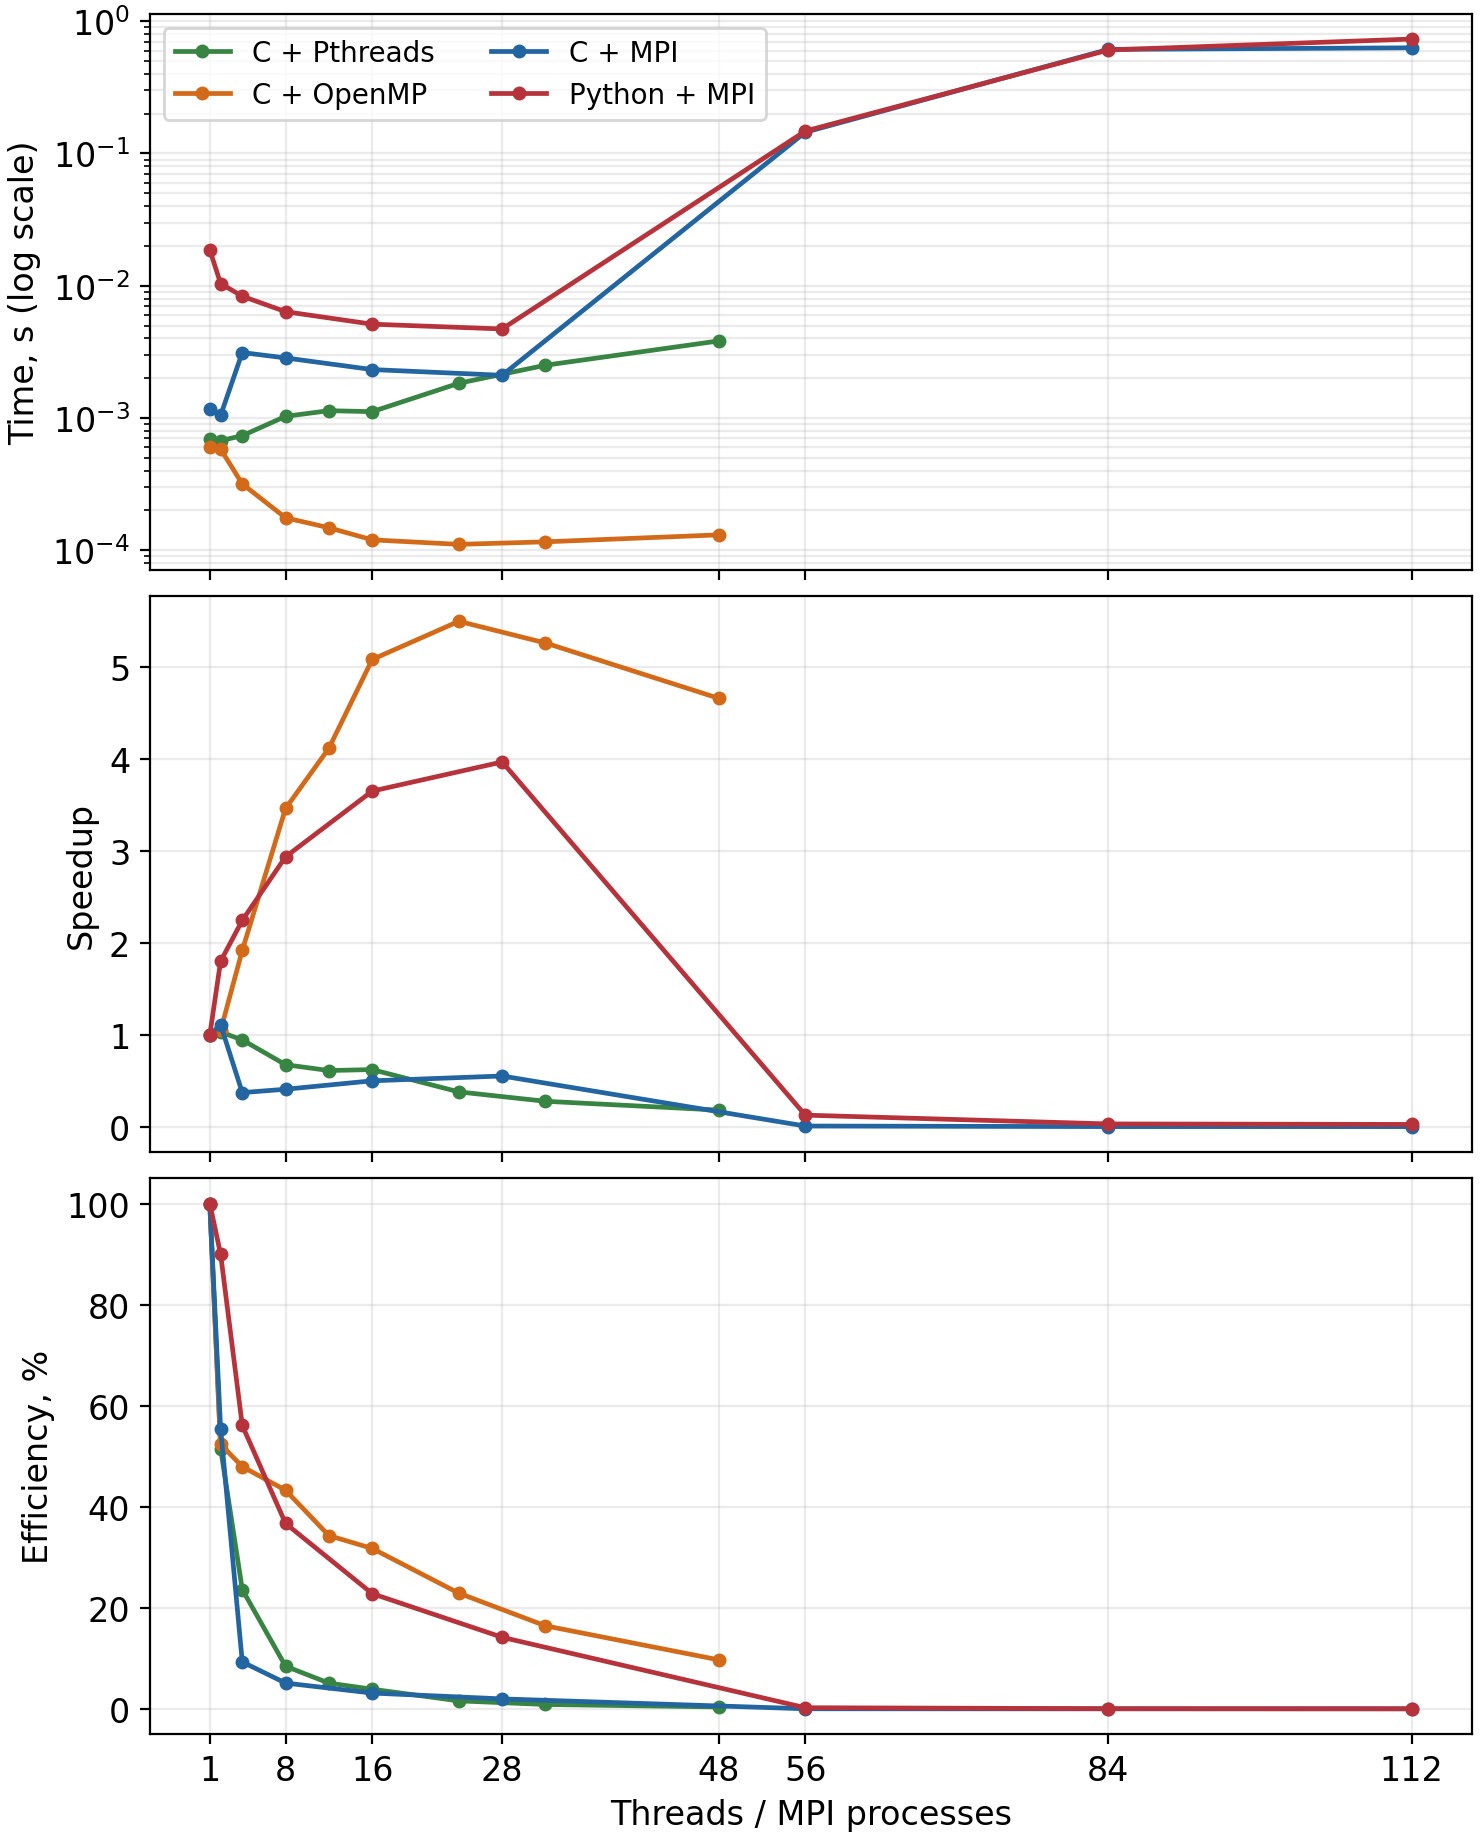
\includegraphics[width=0.94\linewidth,height=0.83\textheight,keepaspectratio]{figures/scaling-10000.png}
\caption{Время, ускорение и эффективность при $n=10\,000$}
\end{figure}
\clearpage
\begin{figure}[p]\centering
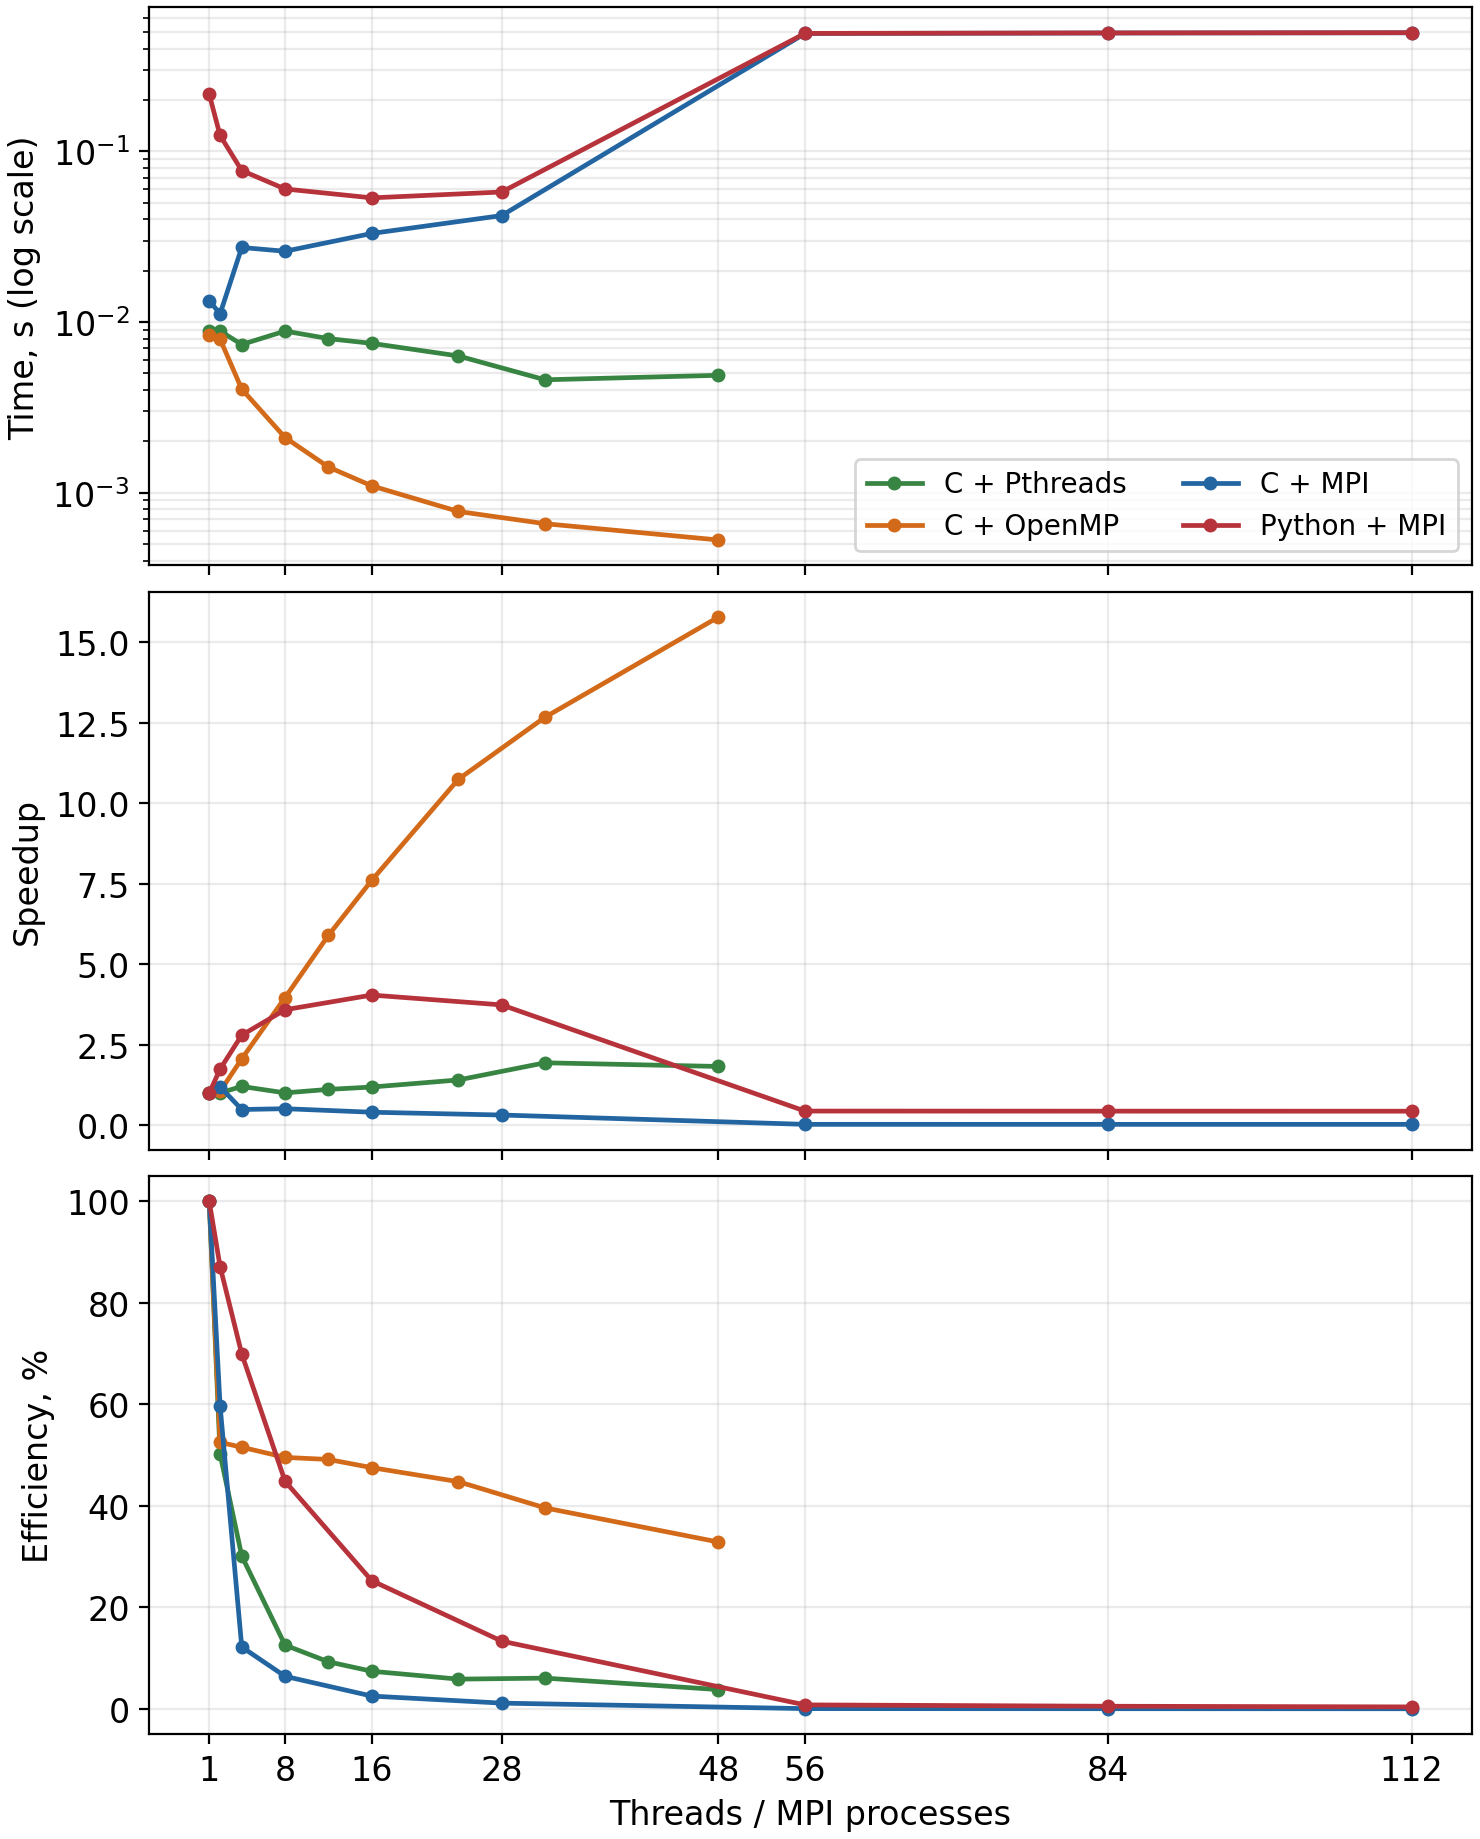
\includegraphics[width=0.94\linewidth,height=0.83\textheight,keepaspectratio]{figures/scaling-100000.png}
\caption{Время, ускорение и эффективность при $n=100\,000$}
\end{figure}
\clearpage
\begin{figure}[p]\centering
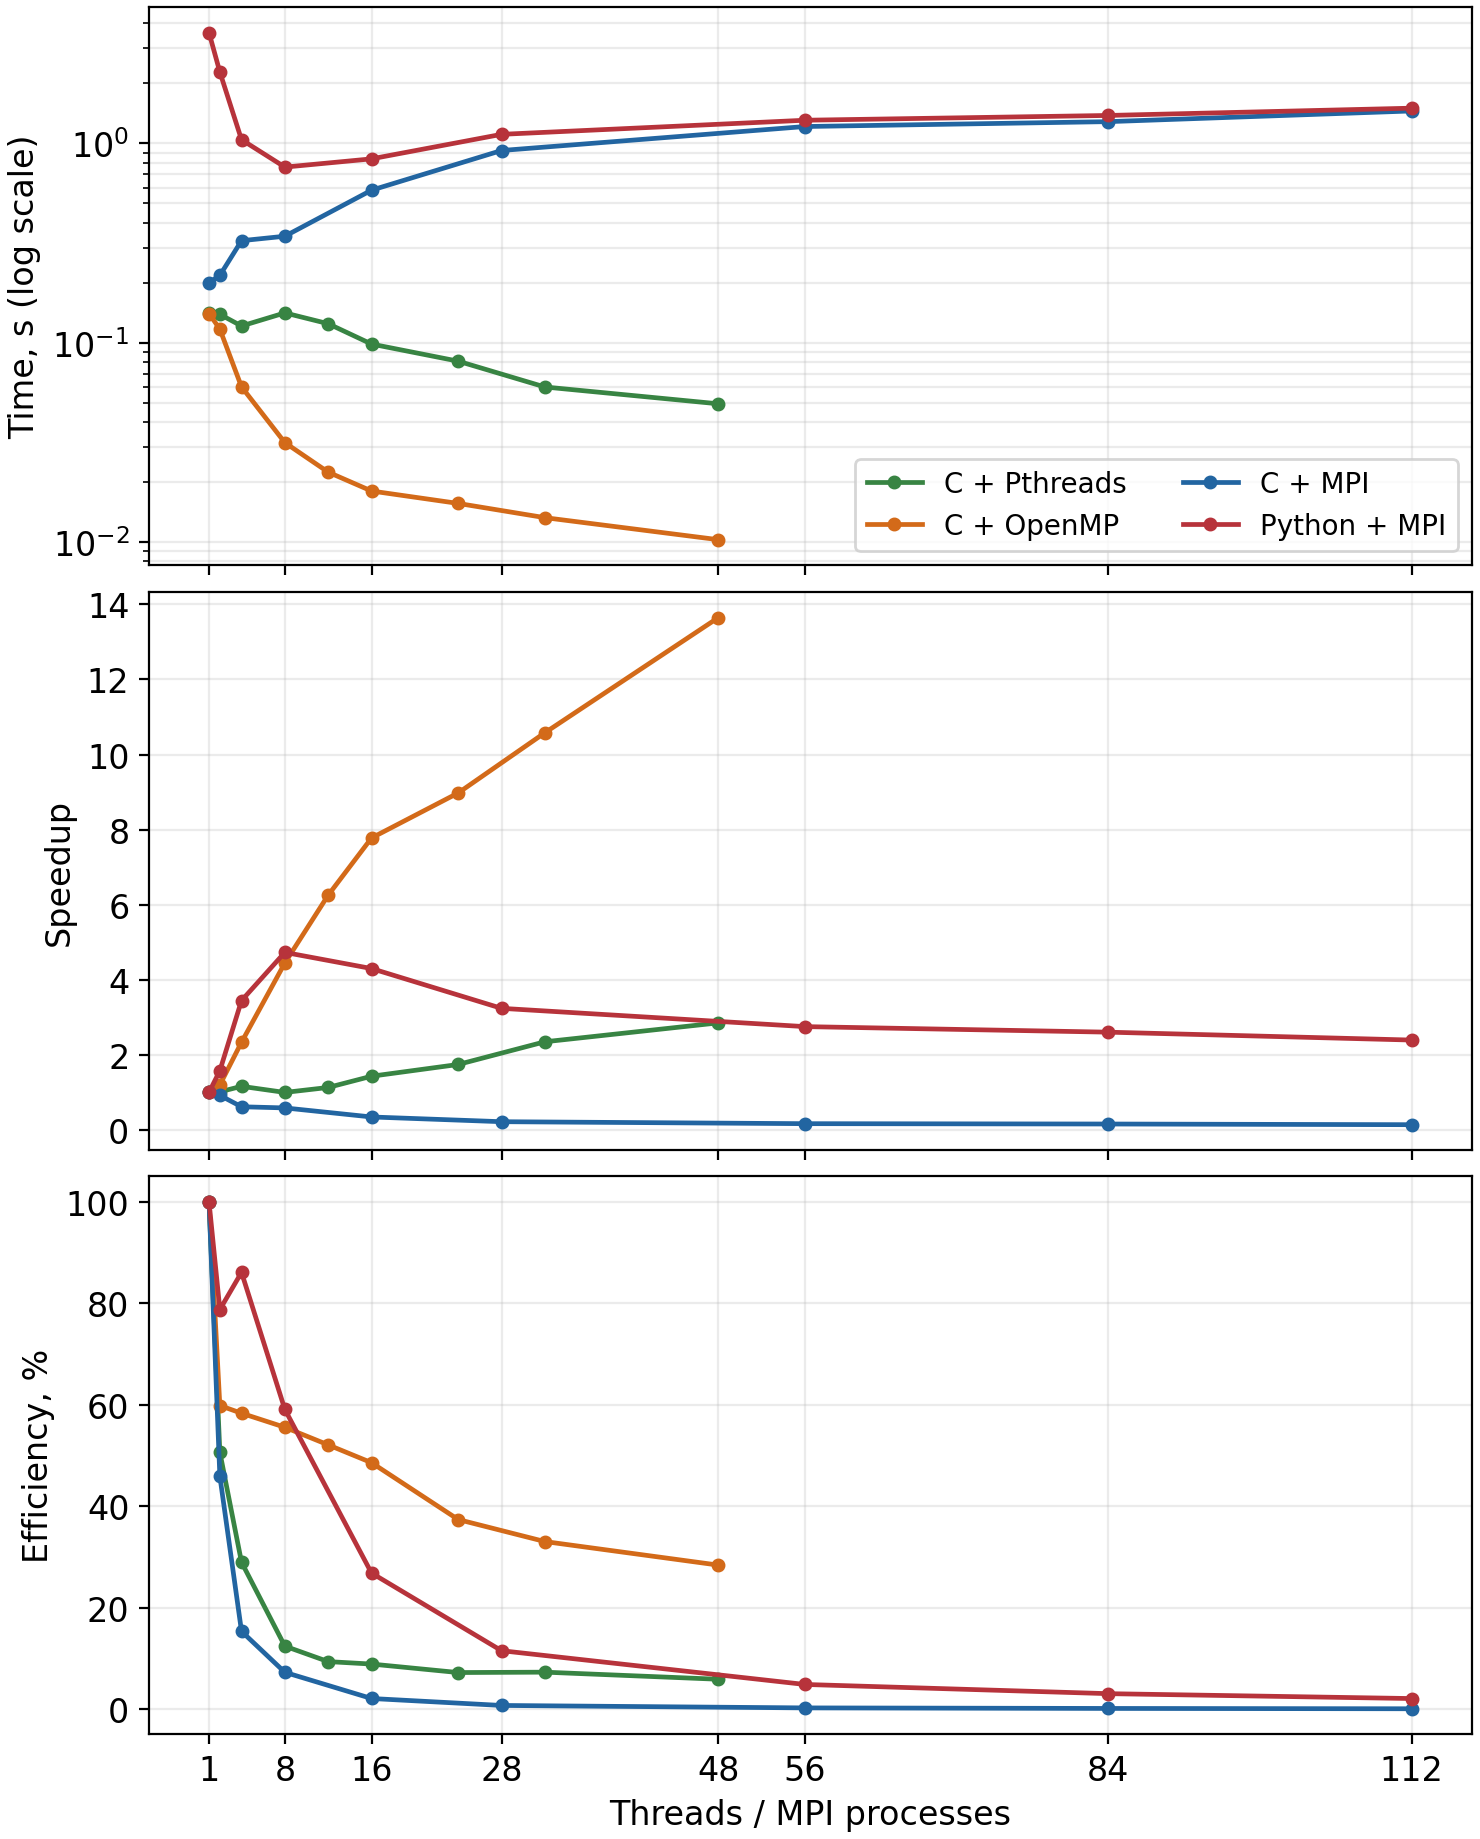
\includegraphics[width=0.94\linewidth,height=0.83\textheight,keepaspectratio]{figures/scaling-1000000.png}
\caption{Время, ускорение и эффективность при $n=1\,000\,000$}
\end{figure}
\clearpage

\section{Заключение}
Реализовано построение натурального кубического сплайна четырьмя способами. Для параллельного решения трёхдиагональной системы применён PCR с $O(\log n)$ стадий и $O(n\log n)$ общей работы. Все реализации прошли разработанный набор тестов относительно SciPy; скриншоты дополнительно подтверждают запуски четырёх версий на вычислительном узле.

Эксперимент до 48 потоков и 112 MPI-процессов показал, что увеличение числа исполнителей не гарантирует ускорения. Лучшие абсолютные времена на всех трёх размерах получены OpenMP. MPI-варианты ограничены репликацией массивов и коллективными обменами; результаты относятся к выбранному TCP-транспорту.

Для дальнейшего улучшения целесообразны блочное распределение строк Pthreads, распределённая редукция с обменом граничными данными, сохранение отдельных повторов и сравнение с последовательной прогонкой. Полученные ускорения характеризуют сравнение с однопоточной или однопроцессной версией того же PCR.

\clearpage\appendix
\section{Команды воспроизведения}
На управляющем сервере:
\begin{samepage}
\par\noindent\begin{minipage}{\linewidth}
\begin{lstlisting}
module load compiler/gcc/11 mpi/openmpi/4.1.6/gcc/11 python/3.10
source ~/spline-lab/.venv/bin/activate
cd ~/spline-lab
make -j3
mkdir -p logs results work
sbatch slurm/threads.sbatch
sbatch slurm/mpi.sbatch
squeue -u "$USER"
\end{lstlisting}
\end{minipage}\par
\end{samepage}
После успешного завершения заданий:
\begin{samepage}
\par\noindent\begin{minipage}{\linewidth}
\begin{lstlisting}
python3 scripts/plot.py
\end{lstlisting}
\end{minipage}\par
\end{samepage}
Для ручной проверки сначала выделить вычислительный узел и перейти на него, затем загрузить модули и активировать окружение. Команды запуска:
\begin{samepage}
\par\noindent\begin{minipage}{\linewidth}
\begin{lstlisting}
export OMPI_MCA_pml=ob1
export OMPI_MCA_btl=self,vader,tcp
export OPENBLAS_NUM_THREADS=1
export MKL_NUM_THREADS=1
python3 scripts/generate.py work/demo.txt --n 129 --case uneven
./bin/spline_pthreads work/demo.txt 4 work/out.txt
python3 scripts/check.py work/demo.txt work/out.txt
./bin/spline_openmp work/demo.txt 4 work/out.txt
python3 scripts/check.py work/demo.txt work/out.txt
mpirun -np 4 ./bin/spline_mpi work/demo.txt 4 work/out.txt
python3 scripts/check.py work/demo.txt work/out.txt
mpirun -np 4 python3 src/spline_mpi.py work/demo.txt 4 work/out.txt
python3 scripts/check.py work/demo.txt work/out.txt
\end{lstlisting}
\end{minipage}\par
\end{samepage}
Новые задания Slurm получат другие номера. Полный набор тестов запускается командой \code{bash tests/correctness.sh} на выделенных ресурсах. После завершения интерактивного сеанса необходимо освободить выделение.

\clearpage
\section{Состав программного проекта}
\begin{table}[H]\centering\small
\begin{tabular}{p{6.1cm}p{8cm}}\toprule
Файл & Назначение\\\midrule
\code{src/spline.c} & Три C-реализации: Pthreads, OpenMP, MPI\\
\code{src/spline_mpi.py} & Python и MPI\\
\code{src/spline_math.py} & Численные функции Python\\
\code{scripts/generate.py} & Генерация исходных точек\\
\code{scripts/check.py} & Проверка относительно SciPy\\
\code{tests/correctness.sh} & Набор кластерных тестов\\
\code{tests/local_math.py} & Локальные проверки численных функций\\
\code{slurm/threads.sbatch} & Серия потоковых запусков\\
\code{slurm/mpi.sbatch} & Серия MPI-запусков\\
\code{scripts/plot.py} & Агрегация результатов и графики\\
\code{results/benchmark.csv} & Полная таблица 108 конфигураций\\
\code{logs/*.out} & Исходные времена запусков\\
\code{intro/transform.py} & Транспонирование JSON-матрицы\\
\code{report/figures/*.png} & Скриншоты запусков\\\bottomrule
\end{tabular}
\end{table}

\begin{thebibliography}{9}
\bibitem{scipy} SciPy. CubicSpline: piecewise cubic interpolation.\\
\url{https://docs.scipy.org/doc/scipy/reference/generated/scipy.interpolate.CubicSpline.html}
\bibitem{mpi} MPI Forum. MPI: A Message-Passing Interface Standard.\\
\url{https://www.mpi-forum.org/docs/}
\bibitem{omp} OpenMP Architecture Review Board. OpenMP API Specifications.\\
\url{https://www.openmp.org/specifications/}
\end{thebibliography}
\end{document}
